\documentclass[12pt,a4paper]{article}

\usepackage[utf8]{inputenc}
\usepackage[T1]{fontenc}
\usepackage[brazil]{babel}
\usepackage{geometry}
\geometry{margin=2.5cm}

\usepackage[final]{graphicx}
\usepackage{float}
\usepackage{caption}
\captionsetup{font=small,labelfont=bf}
\usepackage{hyperref}
\hypersetup{colorlinks=true, linkcolor=black, urlcolor=blue}

\title{Controle-se: Aplicação Web de Controle de Gastos Pessoais\\
\large AED III — Trabalho Prático}
\author{Ana Carolina Couto Machado e Marcos Paulo Da Silva Laine.}
\date{\today}

\begin{document}
\maketitle

\section*{Formulário de Identificação}
\begin{table}[H]
\centering
\begin{tabular}{|l|p{10cm}|}
\hline
\textbf{Disciplina} & Algoritmos e Estruturas de Dados III \\
\hline
\textbf{Professor} & [Nome do Professor] \\
\hline
\textbf{Período} & 2025/1 \\
\hline
\textbf{Alunos} & Ana Carolina Couto Machado e Marcos Paulo Da Silva Laine \\
\hline
\textbf{Matrículas} & [Matrícula Ana] e [Matrícula Marcos] \\
\hline
\textbf{Título do Projeto} & Controle-se: Aplicação Web de Controle de Gastos Pessoais \\
\hline
\textbf{Data de Entrega} & \today \\
\hline
\textbf{Repositório} & \url{https://github.com/marcoslaine/controle-se} \\
\hline
\end{tabular}
\end{table}

\newpage
\part*{Fase I}
\addcontentsline{toc}{part}{Fase I}

\section{Descrição do Problema e Tema}
O \textbf{Controle-se} é uma aplicação web para controle de gastos pessoais. O sistema permite
registrar \textbf{gastos} e \textbf{receitas}, categorizá-los, gerenciar contas (carteira, banco, cartão),
definir orçamentos mensais por categoria e visualizar indicadores (saldo por conta, execução do orçamento e histórico).

\subsection*{Requisitos}
\begin{itemize}
  \item \textbf{Funcionais}: Definição de orçamento; categorização de gasto; inserção, remoção e edição de gasto; \
  inserção de contas bancárias; visualização geral; visualização de gastos recentes; filtrar gastos por categorias
  \item \textbf{Não funcionais}: dados criptografados; armazenamento local; dados comprimidos;
\end{itemize}

\section{Diagrama de Caso de Uso}
\begin{figure}[H]
  \centering
  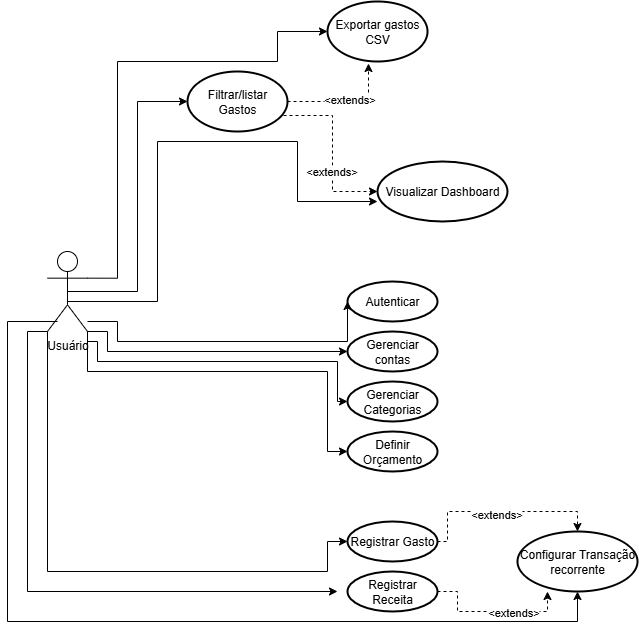
\includegraphics[width=\textwidth,height=.86\textheight,keepaspectratio]{caso.png}
  \caption{Diagrama de Caso de Uso do \textit{Controle-se}.}
\end{figure}

\section{DER Conceitual}
\begin{figure}[H]
  \centering
  \includegraphics[width=\textwidth,height=.86\textheight,keepaspectratio]{DER.png}
  \caption{DER conceitual com relacionamento \textbf{N:N} entre Categoria e Gasto.}
\end{figure}

\section{Aderência aos Requisitos}
\begin{itemize}
  \item \textbf{Mínimo de 3 tabelas além de usuário}: \textit{Conta, Categoria, Gasto, Orçamento e receita}.
  \item \textbf{1:N}: Usuário–Conta; Conta–Gasto.
  \item \textbf{N:N}: \textbf{Categoria–Gasto} via \textit{GASTO\_CATEGORIA}.
  \item \textbf{Tipos}: data (\texttt{Gasto.data}); real (\texttt{Gasto.valor});
        string (vários); \textbf{string multivalorado} representado pela associação N:N (um gasto pode ter lista de categorias) e \textbf{atributo multivalorado nativo} \texttt{Gasto.observacoes} como array de strings.
\end{itemize}

\newpage
\part*{Fase II}
\addcontentsline{toc}{part}{Fase II}

\section{Estruturas de Dados Implementadas}

\subsection{Árvore B+ (Índices Primários)}

A \textbf{Árvore B+} foi implementada como estrutura de indexação primária para todas as tabelas do sistema.
É uma árvore de busca balanceada que mantém os dados ordenados e permite buscas, inserções e remoções eficientes.

\subsubsection*{Características da Implementação}
\begin{itemize}
  \item \textbf{Ordem}: 4 (número máximo de filhos por nó)
  \item \textbf{Número máximo de chaves}: 3 (ordem - 1)
  \item \textbf{Número mínimo de filhos} (nós internos não-raiz): 2 ($\lceil$4/2$\rceil$)
  \item \textbf{Número mínimo de chaves} (nós internos não-raiz): 1 ($\lceil$4/2$\rceil$ - 1)
  \item \textbf{Nós folha}: Armazenam todos os registros de dados e são encadeados para navegação sequencial
  \item \textbf{Nós internos}: Armazenam apenas chaves de roteamento e ponteiros para filhos
  \item \textbf{Balanceamento}: Automático através de divisão e fusão de nós
\end{itemize}

\subsubsection*{Aplicações no Sistema}
\begin{itemize}
  \item \texttt{tabelaUsuarios}: ID\_Usuario $\rightarrow$ Usuario
  \item \texttt{tabelaCategorias}: ID\_Categoria $\rightarrow$ Categoria
  \item \texttt{tabelaGastos}: ID\_Gasto $\rightarrow$ Gasto
  \item \texttt{tabelaReceitas}: ID\_Receita $\rightarrow$ Receita
  \item \texttt{tabelaContas}: ID\_Conta $\rightarrow$ Conta
  \item \texttt{tabelaOrcamentos}: ID\_Orcamento $\rightarrow$ Orcamento
  \item \texttt{tabelaTags}: ID\_Tag $\rightarrow$ Tag
\end{itemize}

\subsubsection*{Operações Implementadas}
\begin{itemize}
  \item \textbf{inserir(chave, dados)}: Inserção com balanceamento automático — O(log n)
  \item \textbf{buscar(chave)}: Busca por chave primária — O(log n)
  \item \textbf{remover(chave)}: Remoção lógica (lápide) — O(log n)
  \item \textbf{buscarIntervalo(inicio, fim)}: Busca por intervalo de chaves — O(log n + m)
  \item \textbf{listarTodos()}: Percurso sequencial nas folhas — O(n)
\end{itemize}

\subsection{Hash Extensível (Índices Secundários e Relacionamentos)}

O \textbf{Hash Extensível} foi implementado para gerenciar relacionamentos 1:N, N:N e índices secundários.
É uma estrutura de hash dinâmica que cresce conforme necessário, mantendo complexidade de busca O(1) médio.

\subsubsection*{Características da Implementação}
\begin{itemize}
  \item \textbf{Capacidade por bucket}: 3 registros
  \item \textbf{Profundidade global}: Número de bits usados para indexar o diretório
  \item \textbf{Profundidade local}: Número de bits usados por cada bucket
  \item \textbf{Crescimento dinâmico}: Diretório duplica quando bucket transborda e profundidades coincidem
\end{itemize}

\subsubsection*{Aplicações no Sistema}

\textbf{Relacionamentos 1:N (Foreign Keys):}
\begin{itemize}
  \item \texttt{indiceUsuarioCategorias}: Usuario $\rightarrow$ Lista<Categoria>
  \item \texttt{indiceUsuarioGastos}: Usuario $\rightarrow$ Lista<Gasto>
  \item \texttt{indiceUsuarioReceitas}: Usuario $\rightarrow$ Lista<Receita>
  \item \texttt{indiceUsuarioContas}: Usuario $\rightarrow$ Lista<Conta>
  \item \texttt{indiceUsuarioOrcamentos}: Usuario $\rightarrow$ Lista<Orcamento>
  \item \texttt{indiceUsuarioTags}: Usuario $\rightarrow$ Lista<Tag>
  \item \texttt{indiceCategoriaOrcamentos}: Categoria $\rightarrow$ Lista<Orcamento>
\end{itemize}

\textbf{Relacionamento N:N:}
\begin{itemize}
  \item \texttt{indiceCategoriaGastos}: Categoria $\rightarrow$ Lista<Gasto>
  \item \texttt{indiceGastoCategorias}: Gasto $\rightarrow$ Lista<Categoria>
  \item \texttt{indiceTagGastos}: Tag $\rightarrow$ Lista<Gasto>
  \item \texttt{indiceGastoTags}: Gasto $\rightarrow$ Lista<Tag>
  \item \texttt{indiceTagReceitas}: Tag $\rightarrow$ Lista<Receita>
  \item \texttt{indiceReceitaTags}: Receita $\rightarrow$ Lista<Tag>
\end{itemize}

\textbf{Índices para Consultas Específicas:}
\begin{itemize}
  \item \texttt{indiceEmailUsuarios}: Hash(Email) $\rightarrow$ Usuario (para login)
  \item \texttt{indiceDataGastos}: Hash(Data) $\rightarrow$ Lista<Gasto> (filtro por data)
  \item \texttt{indiceDataReceitas}: Hash(Data) $\rightarrow$ Lista<Receita> (filtro por data)
  \item \texttt{indiceTipoContas}: Hash(Tipo) $\rightarrow$ Lista<Conta> (filtro por tipo)
\end{itemize}

\subsubsection*{Operações Implementadas}
\begin{itemize}
  \item \textbf{inserir(chave, valor)}: Inserção com divisão de bucket se necessário — O(1) médio
  \item \textbf{buscar(chave)}: Retorna lista de valores associados — O(1) médio
  \item \textbf{remover(chave)}: Remove todas entradas com a chave — O(1) médio
  \item \textbf{expandirDiretorio()}: Duplica diretório quando necessário — O(2^d) onde d = profundidade
\end{itemize}

\section{Análise de Complexidade}

\begin{table}[H]
\centering
\small
\begin{tabular}{|l|c|c|c|}
\hline
\textbf{Operação} & \textbf{Estrutura} & \textbf{Complexidade} & \textbf{Caso} \\
\hline
Busca por ID (chave primária) & Árvore B+ & O(log n) & Pior caso \\
Inserção com nova chave & Árvore B+ & O(log n) & Pior caso \\
Remoção lógica (lápide) & Árvore B+ & O(log n) & Pior caso \\
Busca por intervalo & Árvore B+ & O(log n + m) & m = registros retornados \\
Listagem completa & Árvore B+ & O(n) & Percurso sequencial \\
\hline
Busca por FK ou atributo & Hash Extensível & O(1) & Caso médio \\
Inserção em índice secundário & Hash Extensível & O(1) & Caso médio \\
Remoção de índice secundário & Hash Extensível & O(1) & Caso médio \\
Filtro por categoria & Hash Extensível & O(1 + k) & k = registros da categoria \\
Filtro por data & Hash Extensível & O(1 + k) & k = registros da data \\
Login (busca por email) & Hash Extensível & O(1) & Caso médio \\
\hline
\end{tabular}
\caption{Complexidade temporal das operações implementadas.}
\end{table}

\section{Persistência em Disco}

O sistema implementa persistência de dados utilizando \textbf{serialização Java} para salvar e carregar
as estruturas de dados em arquivos binários \texttt{.db}.

\subsection*{Arquivos de Persistência}
\begin{itemize}
  \item \texttt{usuarios.db}: Tabela de usuários
  \item \texttt{categorias.db}: Tabela de categorias
  \item \texttt{gastos.db}: Tabela de gastos
  \item \texttt{receitas.db}: Tabela de receitas
  \item \texttt{contas.db}: Tabela de contas bancárias
  \item \texttt{orcamentos.db}: Tabela de orçamentos
  \item \texttt{tags.db}: Tabela de tags
  \item \texttt{contadores.db}: Contadores de IDs auto-incrementais
  \item \texttt{categoria\_gasto.db}: Relacionamento N:N entre Categoria e Gasto
  \item \texttt{transacao\_tag.db}: Relacionamento N:N entre Transações (Gastos/Receitas) e Tags
\end{itemize}

\subsection*{Estratégia de Persistência}
\begin{itemize}
  \item \textbf{Salvamento}: Após cada operação de escrita (inserção, atualização, remoção)
  \item \textbf{Carregamento}: Automático na inicialização do servidor
  \item \textbf{Formato}: Serialização Java (ObjectOutputStream/ObjectInputStream)
  \item \textbf{Exclusão lógica}: Registros marcados como \texttt{ativo = false} (lápide)
\end{itemize}

\section{Operações CRUD Implementadas}

\subsection{Usuários}
\begin{itemize}
  \item \textbf{Create}: \texttt{cadastrarUsuario(nome, email, senha)} — verifica unicidade de email
  \item \textbf{Read}: \texttt{buscarUsuario(id)}, \texttt{buscarUsuarioPorEmail(email)}
  \item \textbf{Update}: \texttt{atualizarUsuario(id, novaSenha)}
  \item \textbf{Delete}: Exclusão lógica com \texttt{ativo = false}
  \item \textbf{Auth}: \texttt{autenticarUsuario(email, senha)}
\end{itemize}

\subsection{Categorias}
\begin{itemize}
  \item \textbf{Create}: \texttt{cadastrarCategoria(nome, idUsuario)}
  \item \textbf{Read}: \texttt{buscarCategoria(id)}, \texttt{listarCategoriasPorUsuario(idUsuario)}
  \item \textbf{Update}: \texttt{atualizarCategoria(id, novoNome)}
  \item \textbf{Delete}: \texttt{removerCategoria(id)} — exclusão lógica
\end{itemize}

\subsection{Gastos e Receitas}
\begin{itemize}
  \item \textbf{Create}: \texttt{registrarGasto(...)}, \texttt{registrarReceita(...)}
  \item \textbf{Read}: Busca por ID, por usuário, por categoria, por data
  \item \textbf{Update}: \texttt{atualizarGasto(...)}, \texttt{atualizarReceita(...)}
  \item \textbf{Delete}: Exclusão lógica
  \item \textbf{Filtros}: Combinação de categoria + data usando índices Hash
\end{itemize}

\subsection{Contas Bancárias}
\begin{itemize}
  \item \textbf{Create}: \texttt{cadastrarConta(nome, tipo, saldoInicial, idUsuario)}
  \item \textbf{Read}: \texttt{buscarConta(id)}, \texttt{listarContasPorUsuario(idUsuario)}
  \item \textbf{Update}: \texttt{atualizarConta(id, novoNome, novoSaldo)}
  \item \textbf{Delete}: Exclusão lógica
\end{itemize}

\subsection{Orçamentos}
\begin{itemize}
  \item \textbf{Create}: \texttt{cadastrarOrcamento(valorPlanejado, periodo, idCategoria, idUsuario)}
  \item \textbf{Read}: \texttt{buscarOrcamento(id)}, \texttt{listarOrcamentosPorUsuario(idUsuario)}
  \item \textbf{Update}: \texttt{atualizarOrcamento(id, novoValor)}
  \item \textbf{Delete}: Exclusão lógica
\end{itemize}

\subsection{Tags (Sistema de Etiquetas)}
\begin{itemize}
  \item \textbf{Create}: \texttt{cadastrarTag(nome, cor, idUsuario)} — cria tag personalizada com cor em hexadecimal
  \item \textbf{Read}: \texttt{buscarTag(id)}, \texttt{listarTagsPorUsuario(idUsuario)}
  \item \textbf{Update}: \texttt{atualizarTag(id, novoNome, novaCor)}
  \item \textbf{Delete}: Exclusão lógica
  \item \textbf{Associação}: \texttt{associarTagTransacao(idTransacao, tipoTransacao, idTag)}
  \item \textbf{Consultas}: \texttt{buscarTagsGasto(idGasto)}, \texttt{buscarTagsReceita(idReceita)}
  \item \textbf{Filtros}: \texttt{buscarGastosPorTag(idTag)}, \texttt{buscarReceitasPorTag(idTag)}
\end{itemize}

\noindent \textbf{Características das Tags:}
\begin{itemize}
  \item Sistema de etiquetas personalizáveis para organização de transações
  \item Cada tag possui nome único, cor em formato hexadecimal (ex: \texttt{\#3498db})
  \item Relacionamento N:N com Gastos e Receitas (uma transação pode ter múltiplas tags)
  \item Filtro de transações por tags no frontend para análise rápida
  \item Interface visual com badges coloridos para identificação imediata
\end{itemize}

\section{Arquitetura do Sistema}

O sistema implementa uma arquitetura de três camadas:

\subsection*{Camada 1: Frontend Web}
\begin{itemize}
  \item \textbf{Tecnologia}: HTML5 + CSS3 + JavaScript (ES6+)
  \item \textbf{Responsabilidades}: Interface do usuário, validação de formulários, comunicação com API REST
  \item \textbf{Arquivos}: \texttt{index.html}, \texttt{styles.css}, \texttt{app.js}
\end{itemize}

\subsection*{Camada 2: API REST (Servidor Java)}
\begin{itemize}
  \item \textbf{Tecnologia}: Java 11+ com \texttt{com.sun.net.httpserver.HttpServer}
  \item \textbf{Responsabilidades}: Roteamento de requisições, validação de dados, lógica de negócios
  \item \textbf{Endpoints}: Autenticação, Categorias, Contas, Gastos, Receitas, Orçamentos, Tags, Dashboard
  \item \textbf{Formato}: JSON para entrada e saída
  \item \textbf{Arquivo principal}: \texttt{ControleSeServer.java}
\end{itemize}

\noindent \textbf{Principais Endpoints Implementados:}
\begin{itemize}
  \item \texttt{POST /api/auth/login} — Autenticação de usuário
  \item \texttt{POST /api/categories} — Criar categoria
  \item \texttt{GET /api/categories?userId=X} — Listar categorias do usuário
  \item \texttt{POST /api/expenses} — Registrar gasto (com tags opcionais)
  \item \texttt{POST /api/incomes} — Registrar receita (com tags opcionais)
  \item \texttt{GET /api/transactions?userId=X} — Listar transações (inclui tags)
  \item \texttt{POST /api/tags} — Criar tag personalizada
  \item \texttt{GET /api/tags?userId=X} — Listar tags do usuário
  \item \texttt{PUT /api/tags/\{id\}} — Atualizar tag
  \item \texttt{DELETE /api/tags/\{id\}} — Excluir tag (lógica)
\end{itemize}

\subsection*{Camada 3: Banco de Dados (Estruturas de Dados)}
\begin{itemize}
  \item \textbf{Tecnologia}: Árvore B+ e Hash Extensível implementados manualmente
  \item \textbf{Responsabilidades}: Armazenamento, indexação, busca eficiente, persistência
  \item \textbf{Arquivos}: \texttt{BancoDados.java}, \texttt{ArvoreBPlus.java}, \texttt{HashExtensivel.java}
\end{itemize}

\section{Atributos Multivalorados}

\subsection{Implementação}

\textbf{Atributo Multivalorado Nativo:}
\begin{itemize}
  \item \textbf{Campo}: \texttt{Gasto.observacoes} como \texttt{String[]}
  \item \textbf{Tipo}: Array de strings para múltiplas observações por gasto
  \item \textbf{Persistência}: Via Java Serialization junto com o objeto \texttt{Gasto}
  \item \textbf{Operações}: Adição dinâmica de observações via método \texttt{adicionarObservacao()}
\end{itemize}

\textbf{Relacionamentos N:N (Simulando Multivalorados):}
\begin{itemize}
  \item \textbf{Categoria-Gasto}: Via tabela \texttt{CategoriaGasto}
  \item \textbf{Tag-Transação}: Via tabela \texttt{TransacaoTag}
  \item \textbf{Índices}: Hash Extensível para busca eficiente
  \item \textbf{Integridade}: Chaves estrangeiras para consistência
\end{itemize}

\subsection{Características Técnicas}

\begin{itemize}
  \item \textbf{Serialização}: Arrays nativos preservados na persistência
  \item \textbf{Performance}: Acesso direto sem joins para observações
  \item \textbf{Flexibilidade}: Tamanho dinâmico do array de observações
  \item \textbf{UI}: Campo textarea com separação por vírgula/quebra de linha
\end{itemize}

\section{Testes e Validação}

\subsection*{Cenários Testados}
\begin{itemize}
  \item Cadastro de usuário com email único (validação de duplicação)
  \item Login com credenciais válidas e inválidas
  \item Operações CRUD completas em todas as entidades
  \item Filtros combinados: categoria + data + tags para gastos e receitas
  \item Persistência: reinicialização do servidor mantém dados
  \item Exclusão lógica: registros removidos não aparecem mas permanecem no arquivo
  \item Crescimento dinâmico do Hash Extensível com múltiplas inserções
  \item Balanceamento da Árvore B+ com inserções e remoções
  \item Associação N:N de tags com múltiplas transações
  \item Criação de categoria inline durante cadastro de gasto
  \item Filtro de transações por tags com busca client-side
  \item Atributo multivalorado: múltiplas observações por gasto
  \item Persistência de arrays de strings via serialização
\end{itemize}

\subsection*{Validações Implementadas}
\begin{itemize}
  \item Email único para usuários
  \item IDs auto-incrementais para todas as entidades
  \item Verificação de existência antes de operações de atualização/remoção
  \item Tratamento de exceções em operações de I/O
  \item Validação de relacionamentos (FK válidas)
\end{itemize}

\section{Sistema de Relatórios}

\subsection{Implementação}

O sistema de relatórios foi implementado como uma funcionalidade completa que permite análise detalhada dos dados financeiros do usuário através de dashboards interativos e exportação de dados.

\subsubsection*{Backend (Java)}
\begin{itemize}
  \item \textbf{ReportsHandler}: Novo handler para processar requisições de relatórios
  \item \textbf{Métodos de busca por período}: \texttt{buscarGastosPorPeriodo()} e \texttt{buscarReceitasPorPeriodo()}
  \item \textbf{Exportação de dados}: Métodos para exportar relatórios em CSV e XLSX
  \item \textbf{Análise de dados}: Cálculos de totais, análise por categoria, conta e evolução mensal
\end{itemize}

\subsubsection*{Frontend (JavaScript + Chart.js)}
\begin{itemize}
  \item \textbf{Dashboards interativos}: 4 tipos de visualizações gráficas
  \item \textbf{Controles de período}: Mensal, anual e período personalizado
  \item \textbf{Exportação}: Botões para exportar em CSV ou XLSX
  \item \textbf{Cards de resumo}: Totais de receitas, gastos e saldo do período
\end{itemize}

\subsection{Tipos de Relatórios}

\subsubsection*{Visualizações Implementadas}
\begin{enumerate}
  \item \textbf{Gráfico de Pizza}: Gastos por categoria com percentuais
  \item \textbf{Gráfico de Linha}: Evolução mensal de receitas vs gastos (últimos 12 meses)
  \item \textbf{Gráfico de Barras}: Gastos por conta bancária
  \item \textbf{Lista}: Top 5 maiores gastos do período
\end{enumerate}

\subsubsection*{Períodos Disponíveis}
\begin{itemize}
  \item \textbf{Mensal}: Dados do mês atual
  \item \textbf{Anual}: Dados do ano atual
  \item \textbf{Personalizado}: Usuário define início e fim
\end{itemize}

\subsection{Exportação de Dados}

\subsubsection*{Formatos Suportados}
\begin{itemize}
  \item \textbf{CSV}: Formato de planilha simples, compatível com Excel
  \item \textbf{XLSX}: Formato Excel nativo (simulado com separadores de tabulação)
\end{itemize}

\subsubsection*{Dados Exportados}
\begin{itemize}
  \item Tipo de transação (Gasto/Receita)
  \item Descrição da transação
  \item Valor monetário
  \item Data da transação
  \item Categoria(ies) associada(s)
  \item Conta bancária utilizada
  \item Observações (quando existirem)
\end{itemize}

\subsection{Análise de Dados}

O sistema realiza análises automáticas dos dados financeiros:

\begin{itemize}
  \item \textbf{Totais por período}: Soma de receitas, gastos e saldo
  \item \textbf{Análise por categoria}: Distribuição percentual dos gastos
  \item \textbf{Análise por conta}: Gastos por conta bancária
  \item \textbf{Evolução temporal}: Tendências mensais dos últimos 12 meses
  \item \textbf{Top gastos}: Maiores despesas do período para identificação de padrões
\end{itemize}

\section{Repositório do Projeto}

O código-fonte completo do projeto está disponível publicamente no GitHub:

\begin{center}
\url{https://github.com/marcoslaine/controle-se}
\end{center}

\noindent O repositório contém:
\begin{itemize}
  \item Código-fonte Java completo (estruturas de dados, servidor, banco de dados)
  \item Interface web (HTML, CSS, JavaScript)
  \item Documentação técnica e diagramas
  \item Instruções de compilação e execução
  \item Exemplos de uso e testes
  \item Sistema completo de relatórios com dashboards e exportação
\end{itemize}

\section*{Questionário Técnico - Fase II}

\textbf{a) Qual a estrutura usada para representar os registros?}

Os registros são armazenados em disco usando a seguinte estrutura:

\begin{itemize}
  \item \textbf{Formato}: Arquivos binários \texttt{.db} usando serialização Java nativa
  \item \textbf{Organização}: Um arquivo por entidade (usuarios.db, gastos.db, categorias.db, etc.)
  \item \textbf{Estrutura interna}: Cada arquivo contém uma lista serializada de objetos Java
  \item \textbf{Classes}: Implementam interface \texttt{Serializable} com campos específicos:
    \begin{itemize}
      \item \texttt{Usuario}: id, nome, email, senha, ativo
      \item \texttt{Gasto}: id, idUsuario, valor, descricao, data, observacoes[], ativo
      \item \texttt{Categoria}: id, idUsuario, nome, cor, ativo
      \item \texttt{Tag}: id, idUsuario, nome, cor, ativo
    \end{itemize}
  \item \textbf{Persistência}: Carregamento completo do arquivo na memória, modificação e reescrita
  \item \textbf{Índices}: Mantidos em arquivos separados para busca eficiente (Hash Extensível e B+ Tree)
\end{itemize}

\textbf{b) Como atributos multivalorados do tipo string foram tratados?}

Atributos multivalorados do tipo string foram implementados de duas formas:
\begin{itemize}
  \item \textbf{Nativo}: Campo \texttt{observacoes} na classe \texttt{Gasto} como \texttt{String[]}
  \item \textbf{Simulado via relacionamento N:N}: Categorias de um gasto e tags de uma transação através de tabelas de relacionamento (\texttt{CategoriaGasto} e \texttt{TransacaoTag})
\end{itemize}

\textbf{c) Como foi implementada a exclusão lógica?}

A exclusão lógica foi implementada através do campo booleano \texttt{ativo} presente em todas as entidades. Quando um registro é "excluído", o campo \texttt{ativo} é definido como \texttt{false}, mas o registro permanece no banco de dados. As consultas filtram apenas registros com \texttt{ativo = true}.

\textbf{d) Além das PKs, quais outras chaves foram utilizadas nesta etapa?}

Além das chaves primárias (IDs), foram utilizadas:
\begin{itemize}
  \item \textbf{Chaves estrangeiras}: \texttt{idUsuario} em todas as entidades principais
  \item \textbf{Chaves de relacionamento}: \texttt{idCategoria}, \texttt{idGasto}, \texttt{idTag}, \texttt{idTransacao}
  \item \textbf{Chaves de busca}: \texttt{email} (usuários), \texttt{nome} (categorias, contas, tags)
\end{itemize}

\textbf{e) Quais tipos de estruturas foram utilizadas para cada chave de pesquisa?}

\begin{itemize}
  \item \textbf{Árvore B+ (ordem 4)}: Todas as chaves primárias (IDs) e chaves de busca principais
  \item \textbf{Hash Extensível (3 registros/bucket)}: Relacionamentos 1:N e N:N, índices secundários
  \item \textbf{Índices primários}: Usuários, Categorias, Gastos, Receitas, Contas, Orçamentos, Tags
  \item \textbf{Índices secundários}: Relacionamentos categoria-gasto, tag-transação, usuário-entidades
\end{itemize}

\textbf{f) Como foi implementado o relacionamento 1:N?}

Os relacionamentos 1:N foram implementados através de:
\begin{itemize}
  \item \textbf{Chave estrangeira}: Campo \texttt{idUsuario} em todas as entidades dependentes
  \item \textbf{Navegação}: Busca por \texttt{idUsuario} para recuperar registros relacionados
  \item \textbf{Integridade referencial}: Validação de existência do usuário antes de inserir registros dependentes
  \item \textbf{Exclusão em cascata}: Ao excluir usuário, todos os registros dependentes são marcados como inativos
\end{itemize}

\textbf{g) Como os índices são persistidos em disco?}

\begin{itemize}
  \item \textbf{Formato}: Serialização Java nativa (\texttt{.db} files)
  \item \textbf{Atualização}: Índices são atualizados imediatamente após cada operação de escrita
  \item \textbf{Sincronização}: Salvamento automático após cada modificação (insert, update, delete)
  \item \textbf{Estrutura}: Cada índice é um arquivo separado (ex: \texttt{usuarios.db}, \texttt{categorias.db})
\end{itemize}

\textbf{h) Como está estruturado o projeto no GitHub?}

\begin{itemize}
  \item \textbf{src/}: Código-fonte Java (classes principais, handlers, utilitários)
  \item \textbf{data/}: Arquivos de banco de dados (\texttt{.db})
  \item \textbf{docs/}: Documentação técnica (LaTeX, diagramas)
  \item \textbf{Raiz}: Arquivos frontend (\texttt{index.html}, \texttt{styles.css}, \texttt{app.js})
  \item \textbf{Arquitetura}: Frontend Web + Backend Java + Banco de Dados Customizado
  \item \textbf{Módulos}: Separação clara entre lógica de negócio, persistência e interface
\end{itemize}

\newpage
\part*{Fase III}
\addcontentsline{toc}{part}{Fase III}

\section{Relacionamentos N:N}

\subsection{Implementação dos Relacionamentos Muitos-para-Muitos}

O sistema implementa dois relacionamentos N:N principais através de tabelas de junção:

\subsubsection*{Categoria ↔ Gasto (N:N)}
\begin{itemize}
  \item \textbf{Tabela de Junção}: \texttt{CategoriaGasto}
  \item \textbf{Chaves}: \texttt{idCategoria} e \texttt{idGasto}
  \item \textbf{Propósito}: Permitir que um gasto tenha múltiplas categorias
  \item \textbf{Implementação}: Hash Extensível para indexação eficiente
\end{itemize}

\subsubsection*{Tag ↔ Transação (N:N)}
\begin{itemize}
  \item \textbf{Tabela de Junção}: \texttt{TransacaoTag}
  \item \textbf{Chaves}: \texttt{idTag} e \texttt{idTransacao} (pode ser gasto ou receita)
  \item \textbf{Propósito}: Sistema de tags personalizáveis para categorização flexível
  \item \textbf{Implementação}: Hash Extensível para indexação eficiente
\end{itemize}

\subsection{Estruturas de Dados para N:N}

\subsubsection*{Hash Extensível para Relacionamentos}
\begin{itemize}
  \item \textbf{Capacidade por bucket}: 3 registros
  \item \textbf{Chave composta}: Combinação das chaves estrangeiras
  \item \textbf{Operações}: Inserção, busca e remoção de relacionamentos
  \item \textbf{Complexidade}: O(1) médio para operações de relacionamento
\end{itemize}

\subsection{Operações de Navegação}

\subsubsection*{Busca de Relacionamentos}
\begin{itemize}
  \item \textbf{Gastos por Categoria}: Busca todos os gastos de uma categoria específica
  \item \textbf{Categorias por Gasto}: Busca todas as categorias de um gasto específico
  \item \textbf{Transações por Tag}: Busca todas as transações com uma tag específica
  \item \textbf{Tags por Transação}: Busca todas as tags de uma transação específica
\end{itemize}

\subsubsection*{Integridade Referencial}
\begin{itemize}
  \item \textbf{Validação}: Verificação de existência das entidades antes de criar relacionamentos
  \item \textbf{Exclusão em Cascata}: Remoção automática de relacionamentos quando entidades são excluídas
  \item \textbf{Consistência}: Manutenção da integridade dos dados através de validações
\end{itemize}

\subsection{Interface de Usuário para N:N}

\subsubsection*{Seleção Múltipla de Categorias}
\begin{itemize}
  \item \textbf{Checkboxes}: Interface para seleção de múltiplas categorias em gastos
  \item \textbf{Validação}: Pelo menos uma categoria deve ser selecionada
  \item \textbf{Persistência}: Salvamento automático dos relacionamentos criados
\end{itemize}

\subsubsection*{Sistema de Tags}
\begin{itemize}
  \item \textbf{Criação Dinâmica}: Tags são criadas automaticamente quando utilizadas
  \item \textbf{Associação Múltipla}: Uma transação pode ter múltiplas tags
  \item \textbf{Filtros}: Busca de transações por tags específicas
\end{itemize}

\subsection{Benefícios dos Relacionamentos N:N}

\begin{itemize}
  \item \textbf{Flexibilidade}: Categorização múltipla permite análise mais detalhada
  \item \textbf{Organização}: Sistema de tags oferece categorização personalizada
  \item \textbf{Escalabilidade}: Estruturas eficientes suportam grandes volumes de dados
  \item \textbf{Usabilidade}: Interface intuitiva para gerenciamento de relacionamentos
\end{itemize}

\end{document}
